\section{字符串简介}

\begin{frame}[fragile,allowframebreaks] \ft{\secname}
\lstinputlisting[]{
slide04/code/talkback.c
}
\end{frame}


\begin{frame}[fragile] \ft{\secname}
\begin{lstlisting}
Hi! What's your first name?
xiaoping
xiaoping, what's your weight in kilograms?
60
Well, xiaoping, your volume is 0.06 cubic meters.
Also, your first name has 8 letters,
and we have 40 bytes to store in it.
\end{lstlisting}
\end{frame}

\begin{frame}[fragile] \ft{\secname}
\begin{defn}[]{}
字符串(string)就是一个或多个字符的序列。例如:
\begin{lstlisting}
"Once more you open the door!"
\end{lstlisting}

\end{defn}
\vspace{0.1in}

\begin{free}[注意]{}
字符串用双引号括起来,但双引号不是字符串的一部分。
\end{free}
\end{frame}

\begin{frame} \ft{\secname}

  \begin{free}[C 字符串]{}
    \begin{itemize}
    \item
      C没有为字符串定义专门的数据类型,而是把它存储在 \lstinline|char| 数组中。
      \\[0.1in]
    \item
      字符串的字符存放字符数组中,每个字符占用一个单元。
    \end{itemize}
  \end{free}
  \lstinputlisting[]{slide04/code/greeting.c}
\end{frame}

\begin{frame} \ft{\secname}
  \begin{free}[C++ 字符串]{}
    C++ 提供了两种类型的字符串表示形式:
    \begin{itemize}
    \item
      C 风格字符串
      \\[0.05in]
      \begin{itemize}
      \item C风格的字符串起源于C语言,并在C++中继续得到支持。
      \end{itemize} \vspace{.1in} 
    \item
      C++ 引入的\lstinline|string| 类类型 \\[.05in]
      \begin{itemize}
      \item C++ 标准库提供了 \lstinline|string| 类类型。
      \end{itemize}
    \end{itemize}
  \end{free}

\end{frame}

\begin{frame} \ft{\secname}
  \lstinputlisting[basicstyle=\ttfamily\footnotesize]{slide04/code/greeting1.cpp}
  \lstinputlisting[basicstyle=\ttfamily\footnotesize]{slide04/code/greeting2.cpp}
\end{frame}



% \begin{frame}\ft{\secname}
% \begin{figure}
% \centering
% \begin{tikzpicture}
% \def\x{0.37}
% \foreach \i in {0,1,...,28}{
% \draw[fill=gray!10] (\i*\x,0)rectangle(\i*\x+\x,\x);
% \ifthenelse{\i=0} {\node at (\i*\x+0.5*\x,0) [above]{O};}{}
% \ifthenelse{\i=1} {\node at (\i*\x+0.5*\x,0) [above]{n};}{}
% \ifthenelse{\i=2} {\node at (\i*\x+0.5*\x,0) [above]{c};}{}
% \ifthenelse{\i=3} {\node at (\i*\x+0.5*\x,0) [above]{e};}{}
% \ifthenelse{\i=4} {
% \node at (\i*\x+0.5*\x,0) [above]{ };
% \draw[->,>=stealth,very thick](\i*\x+0.5*\x,-1.2*\x)--(\i*\x+0.5*\x,0);
% \node at (\i*\x+0.5*\x,-2*\x){每个单元占1个字节};

% }{}
% \ifthenelse{\i=5} {\node at (\i*\x+0.5*\x,0) [above]{m};}{}
% \ifthenelse{\i=6} {\node at (\i*\x+0.5*\x,0) [above]{o};}{}
% \ifthenelse{\i=7} {\node at (\i*\x+0.5*\x,0) [above]{r};}{}
% \ifthenelse{\i=8} {\node at (\i*\x+0.5*\x,0) [above]{e};}{}
% \ifthenelse{\i=9} {\node at (\i*\x+0.5*\x,0) [above]{ };}{}
% \ifthenelse{\i=10}{\node at (\i*\x+0.5*\x,0.4*\x) []{y};}{}
% \ifthenelse{\i=11}{\node at (\i*\x+0.5*\x,0) [above]{o};}{}
% \ifthenelse{\i=12}{\node at (\i*\x+0.5*\x,0) [above]{u};}{}
% \ifthenelse{\i=13}{\node at (\i*\x+0.5*\x,0) [above]{ };}{}
% \ifthenelse{\i=14}{\node at (\i*\x+0.5*\x,0) [above]{o};}{}
% \ifthenelse{\i=15}{\node at (\i*\x+0.5*\x,0.4*\x) []{p};}{}
% \ifthenelse{\i=16}{\node at (\i*\x+0.5*\x,0) [above]{e};}{}
% \ifthenelse{\i=17}{\node at (\i*\x+0.5*\x,0) [above]{n};}{}
% \ifthenelse{\i=18}{\node at (\i*\x+0.5*\x,0) [above]{ };}{}
% \ifthenelse{\i=19}{\node at (\i*\x+0.5*\x,0) [above]{t};}{}
% \ifthenelse{\i=20}{\node at (\i*\x+0.5*\x,0) [above]{h};}{}
% \ifthenelse{\i=21}{\node at (\i*\x+0.5*\x,0) [above]{e};}{}
% \ifthenelse{\i=22}{\node at (\i*\x+0.5*\x,0) [above]{ };}{}
% \ifthenelse{\i=23}{\node at (\i*\x+0.5*\x,0) [above]{d};}{}
% \ifthenelse{\i=24}{\node at (\i*\x+0.5*\x,0) [above]{o};}{}
% \ifthenelse{\i=25}{\node at (\i*\x+0.5*\x,0) [above]{o};}{}
% \ifthenelse{\i=26}{\node at (\i*\x+0.5*\x,0) [above]{r};}{}
% \ifthenelse{\i=27}{\node at (\i*\x+0.5*\x,0) [above]{!};}{}

% \ifthenelse{\i=28}{
% \node at (\i*\x+0.5*\x,0) [above]{$\backslash$0};
% \draw[->,>=stealth,very thick](\i*\x+0.5*\x,-1.2*\x)--(\i*\x+0.5*\x,0);
% \node at (\i*\x+0.5*\x,-2*\x){空字符};
% }{}

% }
% \end{tikzpicture}
% \end{figure}
% \end{frame}

\begin{frame}[fragile]\ft{\secname}
  \begin{free}[C字符串]{}
    \begin{itemize}
    \item C字符串存储在字符数组中,最后一个元素为空字符 \lstinline|'\0'|,用于标记字符串的结束。\\[0.15in]
    \item  \lstinline|'\0'| 不是数字0,它是非打印字符,其ASCII码的值为0。\\[0.15in]
    \item \lstinline|'\0'|的存在意味着数组长度至少要比存储字符数多1。
    \end{itemize}    
  \end{free}

\end{frame}


\begin{frame}[fragile]\ft{\secname}
\begin{defn}[数组(array)]{}
\red{数组}是同一类型的数据元素的有序序列。
\end{defn}
\pause

\begin{lstlisting}
char name[40];
\end{lstlisting}
该声明语句创建一个有40个存储单元的数组,其中每个单元可存储一个char型值。
\pause \vspace{0.1in}

\begin{itemize}
\item \lstinline|[]| 说明 \lstinline|name| 是一个数组\\[0.1in]
\item \lstinline|[]| 中的 \lstinline|40| 指出数组的元素个数\\[0.1in]
\item \lstinline|char| 标识每个元素的类型
\end{itemize}
\end{frame}


\begin{frame}[fragile]\ft{\secname:字符串的使用}
  要使用C字符串,必须创建一个数组,把字符串中的字符逐个放入数组中,最后还需在结尾添加一个空字符 \lstinline|'\0'|。 如:
  \begin{lstlisting}
char greeting[10] = {'H', 'e', 'l', 'l', '0', '\0'};    
\end{lstlisting} \pause

但这种方法太麻烦,我们可以通过如下方式来自动完成上述过程:
  \begin{lstlisting}
char greeting[10] = "Hello";
\end{lstlisting}  
\end{frame}

\begin{frame}[fragile]\ft{\secname:字符串的使用}
  \lstinputlisting
  {
    slide04/code/praise1.c
  }
  \pause
  
\begin{lstlisting}[backgroundcolor=\color{red!10}]
What's your name?
Xiaoping Zhang
Hello, Xiaoping. What a super marvelous name!
\end{lstlisting}

\end{frame}

\begin{frame}[fragile]\ft{\secname:字符串的使用}
  \lstinputlisting
  {
    slide04/code/praise1.cpp
  }
  \pause
  
\begin{lstlisting}[backgroundcolor=\color{red!10}]
What's your name?
Xiaoping Zhang
Hello, Xiaoping. What a super marvelous name!
\end{lstlisting}

\end{frame}

\begin{frame}[fragile]\ft{\secname:字符串的使用}

  \begin{free}[C字符串的输入]{}
    \begin{itemize}
    \item 无须把 \lstinline|'\0'| 插入 \lstinline|name| 数组中, \lstinline|scanf()| 会在读取输入时完成此任务。\\[0.1in]
    \item  \lstinline|name| 前无须加 \lstinline|&|,因 \lstinline|name| 本身就表示地址。 \\[0.1in]
    \item 使用 \lstinline|%s| 的  \lstinline|scanf()|  语句会在遇到的第一个空格、制表符或换行符处停止读取,它只会把第一个单词而不是把整条语句作为字符串读入。\\[0.1in]
    \end{itemize}
  \end{free}

  \begin{free}[C++字符串的输入]{}
    \begin{itemize}
    \item 使用 \lstinline|cin| 读取字符串时,也按单词读取,即遇到第一个空格、制表符或换行符时会自动忽略后面的内容。\\[0.1in]
    \end{itemize}
  \end{free}

\end{frame}

\begin{frame}[fragile]\ft{\secname:字符与字符串}
  \begin{free}[\lstinline|"x"| 与 \lstinline|'x'| 的差别]{}
    \begin{itemize}
    \item  \lstinline|'x'| 为字符,而 \lstinline|"x"| 为字符串\\[0.1in]
    \item  \lstinline|"x"| 由两个字符 \lstinline|'x'| 和 \lstinline|'\0'| 组成
    \end{itemize}    
  \end{free}

\end{frame}

\begin{frame}[fragile]\ft{\secname:字符串长度}

  \begin{free}[C字符串]{}
    若使用字符数组来存储字符串 \lstinline|char name[40] = "Hello";|,则
    \begin{itemize}
    \item \lstinline|sizeof name| 将 \lstinline|name| 数组所占空间的字节大小,即 40;
    \item 使用\lstinline|strlen(name)| 统计字符串 \lstinline|name| 的字符个数,不包含 \lstinline|'\0'|,即 5。
    \end{itemize}  
  \end{free}


  \begin{free}[C++字符串]{}
    若使用字符串对象 \lstinline|string name = "Hello";|,则
    \begin{itemize}
    \item \lstinline|sizeof| 计算 \lstinline|name| 对象所占空间的字节大小;\\[0.1in]
    \item 使用类方法 \lstinline|name.size()| 来统计字符串的字符个数,不包含 \lstinline|'\0'|,即5。
    \end{itemize}  
  \end{free}
\end{frame}

\begin{frame}\ft{\secname:字符串长度}
\lstinputlisting[]
{
  slide04/code/praise2.c
}
\end{frame}

\begin{frame}[fragile]\ft{\secname}

\begin{lstlisting}[backgroundcolor=\color{red!20}]
What's your name?
Xiaoping
Hello, Xiaoping. What a super marvelous name!
Your name of 8 letters occupied 40 memory cells.
PRAISE has 30 letters and occpied 31 memory cells.
\end{lstlisting}
\end{frame}


\begin{frame}[allowframebreaks]\ft{\secname:字符串长度}
\lstinputlisting[]
{
  slide04/code/praise2.cpp
}
\end{frame}

\begin{frame}[fragile]\ft{\secname:字符串长度}

\begin{lstlisting}[backgroundcolor=\color{red!20}]
What's your name?
Xiaoping
Hello, Xiaoping. What's a super marvelous name!
Your name of 8 letters occupies 32 memory cells.
PRAISE has 30 letters and occupies 31 memory celss.
\end{lstlisting}
\end{frame}


\begin{frame}[fragile]\ft{\secname:字符串函数}
\begin{itemize}
\item \tf 头文件string.h包含许多与字符串相关的函数的原型,包括strlen函数。\\[0.1in]
\item C把函数库分成多个相关函数的序列,并为每个序列提供一个头文件。比如:\\[0.1in]
\item[(1)] printf和scanfs属于标准输入输出序列,使用stdio.h。\\[0.1in]
\item[(2)] strlen和其它一些与字符串相关的函数同属一个系列,使用string.h。
\end{itemize}
\end{frame}

\begin{frame}[fragile]\ft{\secname:printf函数处理长字符串}
\begin{itemize}
\item 一条printf语句占用两行,但只能在参数之间断行,不允许在字符串中间断行。\\[0.1in]
\item 使用两个printf语句输出一行,换行符只出现在第二条语句。
\end{itemize}
\end{frame}

\begin{frame}[fragile]\ft{\secname:sizeof运算符与strlen返回值}
设name = "Morgan",则
\begin{lstlisting}[backgroundcolor=\color{red!10}]
sizeof name : 40
strlen(name): 6
\end{lstlisting}

\begin{figure}
\centering
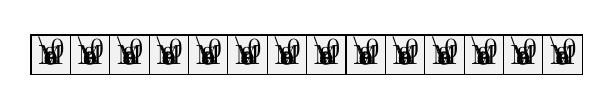
\begin{tikzpicture}
\def\x{0.5}
\foreach \i in {0,1,...,13}{
\draw[fill=gray!10] (\i*\x,0)rectangle(\i*\x+\x,\x);
\ifthenelse{\i=0} {\node at (\i*\x+0.5*\x,0) [above]{M};}{}
\ifthenelse{\i=1} {\node at (\i*\x+0.5*\x,0) [above]{o};}{}
\ifthenelse{\i=2} {\node at (\i*\x+0.5*\x,0) [above]{r};}{}
\ifthenelse{\i=3} {\node at (\i*\x+0.5*\x,0) [above]{g};}{}
\ifthenelse{\i=4} {\node at (\i*\x+0.5*\x,0) [above]{a};}{}
\ifthenelse{\i=5} {\node at (\i*\x+0.5*\x,0) [above]{n};}{}
\ifthenelse{\i=6} {\node at (\i*\x+0.5*\x,0) [above]{$\backslash$0};}{}
\ifthenelse{\i=7} {\node at (\i*\x+0.5*\x,0) [above]{};}{}
\ifthenelse{\i=8} {\node at (\i*\x+0.5*\x,0) [above]{};}{}
\ifthenelse{\i=9} {\node at (\i*\x+0.5*\x,0) [above]{};}{}
\ifthenelse{\i=10}{\node at (\i*\x+0.5*\x,0.4*\x) []{};}{}
\ifthenelse{\i=11}{\node at (\i*\x+0.5*\x,0) [above]{};}{}
\ifthenelse{\i=12}{\node at (\i*\x+0.5*\x,0) [above]{};}{}
\ifthenelse{\i=13}{\node at (\i*\x+0.5*\x,0) [above]{ };}{}
}
\end{tikzpicture}
\end{figure}
\end{frame}

\begin{frame}[fragile]\ft{\secname:sizeof运算符与strlen返回值}
\begin{lstlisting}[backgroundcolor=\color{red!10}]
sizeof PRAISE : 29
strlen(PRAISE): 28
\end{lstlisting}

sizeof运算符在处理字符串变量时,会将空字符也计算在内。
\end{frame}

\begin{frame}[fragile]\ft{\secname:sizeof运算符后的圆括号}
\begin{itemize}
\item 圆括号对于数据类型是必需的,而对于具体量则是可选的。
\begin{lstlisting}[backgroundcolor=\color{red!10}]
sizeof(float)
sizeof(char)

sizeof name
sizeof 2.15
\end{lstlisting}
\item 建议在所有情况下都使用圆括号。
\begin{lstlisting}[backgroundcolor=\color{red!10}]
sizeof(name)
sizeof(2.15)
\end{lstlisting}
\end{itemize}
\end{frame}

